\documentclass[../../TAU.tex]{subfiles}
\begin{document}

\chapter{Основные понятия, структура и классификация систем автоматического управления}

 С древних времен человек хотел использовать предметы и силы природы в своих целях, то есть управлять ими. Теория управления пытается ответить на вопрос «как нужно управлять?». До XIX века науки об управлении не существовало, хотя первые системы автоматического управления уже были (например, ветряные мельницы «научили» разворачиваться навстречу ветру). Развитие теории управления началось в период промышленной революции. Сначала это направление в науке разрабатывалось механиками для решения задач регулирования, то есть поддержания заданного значения частоты вращения, температуры, давления в технических устройствах (например, в паровых машинах). Отсюда происходит название «теория автоматического регулирования». Позднее выяснилось, что принципы управления можно успешно применять не только в технике, но и в биологии, экономике, общественных науках.

\section {Процессы управления}
%Процессы управления (слайд 3) - понятия, общая информация о процессах + таблица

Процессы управления и обработки информации в системах любой природы изучает наука кибернетика. Один из ее разделов, связанный главным образом с техническими системами, называется теорией автоматического управления. 

\begin{table}
\begin{center}

\begin{tabular}{|p{6.5cm}|p{6.5cm}|}
  % after \\: \hline or \cline{col1-col2} \cline{col3-col4} ...
  \hline
  {\bf В живой природе} & {\bf В неживой природе} \\ [4pt]
  \hline 
  Естественный отбор & Наведение на цель орудия \\
  \hline
  Терморегуляция у животных & Поддержание температуры в печи\\
  \hline
  Поддержание равновесия животными & Поддержание равновесия робота\\
  \hline
  Увеличение рождаемости в стране & Поддержание скорости на моторе\\
  \hline
  Уничтожение клеток определенного типа (вирусных, инфекционных и т.п.)& Поддержание фиксированной высоты летального аппарата\\
  \hline
  Повышение работоспособности работников предприятия & Поддержание заданного напряжения\\
  \hline
\end{tabular}
\caption{\it Процессы управления}
\end{center}
\end{table}

\section{Характеристика процессов управления}
%Характеристика процессов управления (слайд 4) - пара слов о каждой характеристике + примеры

Общие характеристики всех процессов управления:
\begin{itemize}
  \item Прием информации - поиск и обнаружение сигналов (выделение сигналов из шума). Примеры: камера, глаз, датчики давления, скорости, положения и т.п., общение.
  \item Хранение информации - процесс поддержания исходной информации в виде, обеспечивающем выдачу данных по запросам конечных пользователей. Примеры: память животных, память на носителях - USB, HDD, CD, DVD.
  \item Преобразование информации - процесс изменения формы представления информации или ее содержания. Примеры: анализ рынка, те или иные вычисления.
  \item Выработка управляющего воздействия - воздействие на объект управления, направленное на достижение цели управления. Примеры: подача напряжения на мотор, передача указаний подчиненным, поворот руля. %-не очень понятно, уточнить.
\end{itemize}

\section{Исходные положения ТАУ}
\subsubsection{САУ. Структурная схема и понятия}
%САУ. Структурная схема и понятия (слайд 5-6) - схема, описание, термины. Что входит в схему, как работает, назначение каждого элемента

\defi{\it Управление} - целенаправленное воздействие не объект или устройство. Управление может быть автоматическим, т.е. без участия человека, ручным, т.е. в присутствии человека, или полуавтоматическим, т.е. работающим при участии человека.

\defi{\it Объект управления} (ОУ) - устройство, которым нужно и можно управлять. Это может быть автомобиль, самолет электродвигатель и т.д.

\defi{\it Цель управления} ОУ - поддержание 
\textit{заданного} 
режима, т. е. изменение какого-либо параметра ОУ по заданному закону (например температура в холодильнике должна быть зафиксированной). Такой параметр называют 
\textit{управляемой} или 
\textit{выходной} переменной. 

\defi{\itСистема автоматического управления} (САУ) - устройство управления (УУ) и объект управления (ОУ).\par
Основной задачей автоматического управления является поддержание определенного закона изменения одной или нескольких физических величин, характеризующих процессы, протекающие в ОУ, без непосредственного участия человека. Эти величины называются {\it управляемыми величинами}. Если в качестве ОУ рассматривается хлебопекарная печь, то управляемой величиной будет температура, которая должна изменяться по заданной программе в соответствии с требованиями технологического процесса. 



\begin{figure}[h]
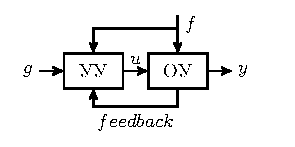
\includegraphics[width=10cm]{SAU_scheme.pdf}
\caption{На структурной схеме САУ: $y$ --- выходная переменная; $g$ --- задающее воздействие (иногда изображается как выход задающего устройства); $f$ --- возмущение, действующее на ОУ и, возможно, на УУ; $u$ --- управление (управляющее воздействие). Канал связи, по которому поступает информация в УУ о состоянии ОУ, называется {\it обратной связью} (feedback). В САУ обратная связь может отсутствовать.}
\centering
\end{figure}

\subsubsection{Понятие устойчивости}
ОУ в зависимости от входных воздействий бывают устойчивые, нейтральные и неустойчивые. Например, пусть при постоянных $u = u_0, f = f_0$ на выходе $y = y_0$. Положим, что на какое-то время $T$ значение $u$ и $f$ изменились, а затем вернулись к исходным значениям. Тогда объект управления

\begin{itemize}
    \item устойчивый, если при $t \rightarrow \infty$ выход $y \rightarrow y_0$; \\
Например, холодильник, генератор напряжения, маятник, унитаз.
    \item нейтральный, если при $t \rightarrow \infty$ выход $y \rightarrow y_1$ и $y_1\neq y_0$. \\
Например, резервуар с водой;
    \item неустойчивый, в противном случае.\\
Самолет с обратной стреловидностью крыла, обратный (перевернутый) маятник.
\end{itemize}

\defi{\it Устойчивость} - это свойство системы возвращаться в установившееся состояние после того, как она была выведена из этого состояния каким-либо возмущением. 
\section{Принципы управления}
В основе построения систем автоматического управления лежат некоторые общие фундаментальные принципы управления, определяющие,каким образом осуществляется увязка алгоритмов управления с заданным и фактическим функционированием, а иногда и с причинами, вызвавшими отклонение.\par
Принято различать три фундаментальных принципа управления: программное управление, принцип компенсации и принцип обратной связи.

\subsubsection{Программное управление}

Управление $u$ выбирается в виде некоторой функции времени $u = u(t)$.

\begin{figure}[h]
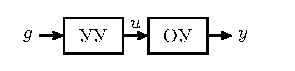
\includegraphics[width=10cm]{program.pdf}
\caption{Программное управление}
\centering
\end{figure}

Условиями применимости этого принципа является наличие полной информации об ОУ, а также --- его устойчивость и отсутствие существенных неизвестных возмущений.

\subsubsection{Принцип компенсации}
Если возмущающий фактор искажает выходную величину до недопустимых пределов, то применяют принцип компенсации. \par
Положим, что начальное значение выходной величины - $g$. Из-за возмущения $f$ на выходе регистрируется значение $у$, которое отклоняется от заданной величины на $u$. 
Если каким-то образом удается измерить величину $f$, то можно откорректировать управляющее воздействие u на входе ОУ, суммируя сигнал УУ с корректирующим воздействием, пропорциональным возмущению $f$ и компенсирующим его влияние.\\\\
{\bf Достоинство принципа компенсации:} быстрота реакции на возмущение. \\
{\bf Недостаток принципа компенсации:} невозможность учета подобным образом всех возможных возмущений.

\subsubsection{Принцип обратной связи (принцип Ползунова - Уатта)}
Один из самых универсальных методов управления, так как не требует информации о возмущениях и условие устойчивости исходного объекта не обязательно.


\begin{figure}[h]
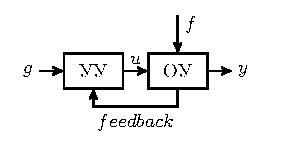
\includegraphics[width=10cm]{feedback.pdf}
\caption{Обратная связь}
\centering
\end{figure}

{\bf Недостаток принципа обратной связи:} невозможность полной компенсации возмущения, в определенных случаях может сделать замкнутую систему неустойчивой. \\
{\bf Достоинством принципа обратной связи:} его универсальность, возможность его использования в условиях отсутствия информации о возмущающих воздействиях. Принцип широко используется в технике, а также присущ живым организмам и обществу.

% TODO ссылку на Емельянова, Коровина

\subsubsection{Принцип комбинированного управления.}
Данный принцип управления применим при одновременном использовании способов управления как по возмущению, так и по отклонению.

\section{АСУ}

{\it Автоматизированные системы управления} (АСУ) включают разнообразные элементы, играющие различную роль в решении задач управления. Выделение отдельных элементов осуществляется в соответствии с их специфическими чертами и вытекающими из этого особенностями разработки и включения в АСУ. 

\begin{figure}[h]
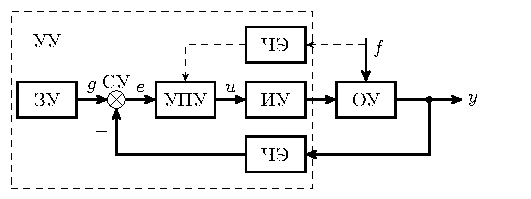
\includegraphics[width=10cm]{SAU_structure.pdf}
\caption{На схеме: 
ЧЭ, чувствительный элемент, измеряющий возмущения (не всегда присутствует)
 и выход $y$; УПУ, усилительно-преобразовательное устройство, вырабатывающее управление $u$ на основе задающего воздействия $g$ и, возможно, измерения $f$; ИУ, исполнительное устройство, которое непосредственно воздействует на ОУ; СУ, сравнительное устройство, вычисляющее отклонение $e$; ЗУ, задающее устройство, вырабатывающее задающее воздействие $g$.}
\centering
\end{figure}


\section{Классификация САУ}
Для ознакомления с основными видами систем автоматического управления и соответствующей терминологией рассмотрим классификацию САУ по ряду признаков, существенных с точки зрения теории автоматического управления. 

\subsubsection{Наличие обратной связи}
По наличию обратной связи САУ делятся на {\it замкнутые} (с обратной связью) и {\it разомкнутые} (без обратной связи).\par
В {\it разомкнутых} САУ выходная величина объекта у не измеряется, т. е. нет контроля за состоянием объекта. Разомкнутыми такие системы называются потому, что вследствие этого в них отсутствует обратная связь между выходом объекта и входом управляющего устройства, при наличии которой объект и управляющее устройство образуют замкнутый контур. \par
В {\it замкнутых} САУ на вход управляющего устройства подаются задающее воздействие $g$ и выходная величина объекта $у$. Исходя из величины $g$, управляющее устройство определяет соответствующее требуемое значение $y$ и, имея информацию о текущем значении $e$, обеспечивает необходимое соответствие между $y$ и $g$ путем воздействия на объект. При этом УУ создает обратную связь вокруг объекта, связывая его выход со входом. Эти системы могут обеспечить принципиально неограниченную точность управления и представляют собой основной тип САУ. 

\subsubsection{Вид задающего воздействия}
В зависимости от вида задающего воздействия САУ делятся на три вида: {\it системы стабилизации}, {\itсистемы программного управления} и {\it системы слежения}. \par
В {\it системах стабилизации} задающее воздействие постоянно ($g = const$), в {\it системах программного управления} оно изменяется по заранее заданному закону ($g = g(t)$ - заданная функция), в {\it системах слежения} задающее воздействие тоже изменяется, но закон изменения заранее не известен, а задающее воздействие определяется внешними факторами (например радиолокация).

\subsubsection{Способ использования текущей информации}
САУ также делятся на \par
{\it неадаптивные}, т.е.  те, в которых текущая информация используется только для выработки управляющего воздействия \par
{\it адаптивные}, т.е. те, в которых текущая информация используется еще и для изменения алгоритма управления или его параметров\\\par
Область применения {\it адаптивных} САУ – это управление объектами, свойства или условия работы которых недостаточно известны или существенно непостоянны. В этих условиях обыкновенная, {\it неадаптивная}, система либо будет работать неудовлетворительно, либо потребует постоянного надзора. 

\subsubsection{Виды сигналов}

САУ бывают {\it непрерывного} или {\it дискретного} действия в зависимости от характера действия составляющих систему звеньев. \par
Система {\it непрерывного} действия состоит только из звеньев непрерывного действия, т. е. звеньев, выходная величина которых изменяется плавно при плавном изменении входной величины. \par
Система {\it дискретного}  действия – это система, содержащая хотя бы одно звено дискретного действия. Звеном дискретного действия называется звено, выходная величина которого изменяется дискретно, т. е. скачками, даже при плавном изменении входной величины.

\subsubsection{Виды уравнения - линейные и нелинейные}

{\it Линейной} называется система, которая описывается линейными уравнениями. В противном случае система является {\it нелинейной} . Чтобы система была {\it нелинейной}, достаточно иметь в ее составе хотя бы одно нелинейное звено, т. е. звено, описываемое нелинейным уравнением. \par
Для {\it линейных} систем справедлив принцип суперпозиции . Он заключается в том, что реакция системы на любую комбинацию внешних воздействий равна сумме реакций на каждое из этих воздействий, поданных на систему порознь. К {\it нелинейным} системам принцип суперпозиции не применим. 


\subsubsection{Характер внешних воздействий}

Система является {\it детерминированной}, если приложенные к ней воздействия и параметры модели являются постоянными, или детерминированными, т.е. определенными, функциями переменных состояния и времени. Систему называют {\it стохастической}, если приложенные к ней воздействия и параметры модели являются случайными функциями или случайными величинами.

\section{Законы управления}
Термин “закон управления” перешел в теорию управления из классической теории. 

\defi{\it Закон управления} - математическая зависимость, по которой управляющее устройство воздействовало бы на объект, если бы оно было безынерционным. Законы управления используются в промышленных регуляторах (манипуляторах, станках и пр.). Основными законами управления являются: П-закон, ПИ-закон, ПД-закон, ПИД-закон.

\subsubsection{П-закон}

{\it Пропорциональный закон (П-закон)} - линейный закон, осуществляемый с помощью П-регулятора (статический регулятор), отражающий прямо пропорциональную зависимость между изменением управляющего воздействия и погрешностью $е$ регулирования.. \par
П-закон имеет вид $u = k_{\text{п}} e$.  Постоянная $k_{\text{п}}$ - коэффициент передачи (пропорциональности, усиления) регулятора, а обратная ему величина $\delta\text{п}=\frac{1}{k_{\text{п}}}$- статистизм регулятора.  \par
П-регуляторы применяются для управления объектами с самовыравниванием и без самовыравнивания при небольших изменениях нагрузок. 


\subsubsection{ПИ-закон}

{\it Пропорционально-интегральный закон (ПИ-закон)} - закон, осуществляемый с помощью ПИ-регулятора и имеющий вид $u=k_\text{п}e+ k_\text{и}\int\limits_0^t e(t) dt$.  Регулирование частоты синхронных генераторов выполняется путем двойного проверки: статическим регулятором скорости турбины и астатистической коррекцией, вводимой регулятором частоты электрического тока. \par
ПИ-регулятор является наиболее распространенным на практике, так как достаточно прост в настройке и обеспечивает нулевую статическую ошибку регулирования. Данный тип регуляторов применяют для регулирования как устойчивых, так и нейтральных объектов при больших, но плавных изменениях нагрузок, когда требуется высокая точность регулирования в статическом режиме (когда остаточные отклонения недопустимы).


\subsubsection{ПИД-закон}

{\it Пропорционально-интегрально-дифференциальный закон (ПИД-закон)} осуществляется с помощью ПИД-регулятора, который обеспечивает астатистическое регулирование. ПИД-закон имеет вид $u=k_\text{п}e+ k_\text{и}\int\limits_0^t e(t) dt +k_\text{д} \frac{de(t)}{dt}$ Производная $\frac{d e(t)}{dt}$ вводится в закон регулирования с целью повышения качества процесса регулирования. Постоянные $k_\text{и}$ и $k_\text{д}$ - постоянные времени интегрирования и дифференцирования соответственно. ПИД-регуляторы.
ПИД-регуляторы обеспечивают относительно высокое качество регулирования объектов, обладающих переходным запаздыванием (например теплообменных и массообменных аппаратов), а так же в тех случаях, когда нагрузка в объектах регулирования изменяется часто и быстро.


\subsubsection{ПД-закон}

{\it Пропорционально-дифференциальный закон (ПД-закон)}, осуществляемый с помощью ПД-регуляторов, имеет вид $u=k_\text{п}e+ k_\text{д} \frac{de(t)}{dt}$. ПД-уравнения применяются для повышения быстродействия работы системы.

\begin{figure}[h]
\centering
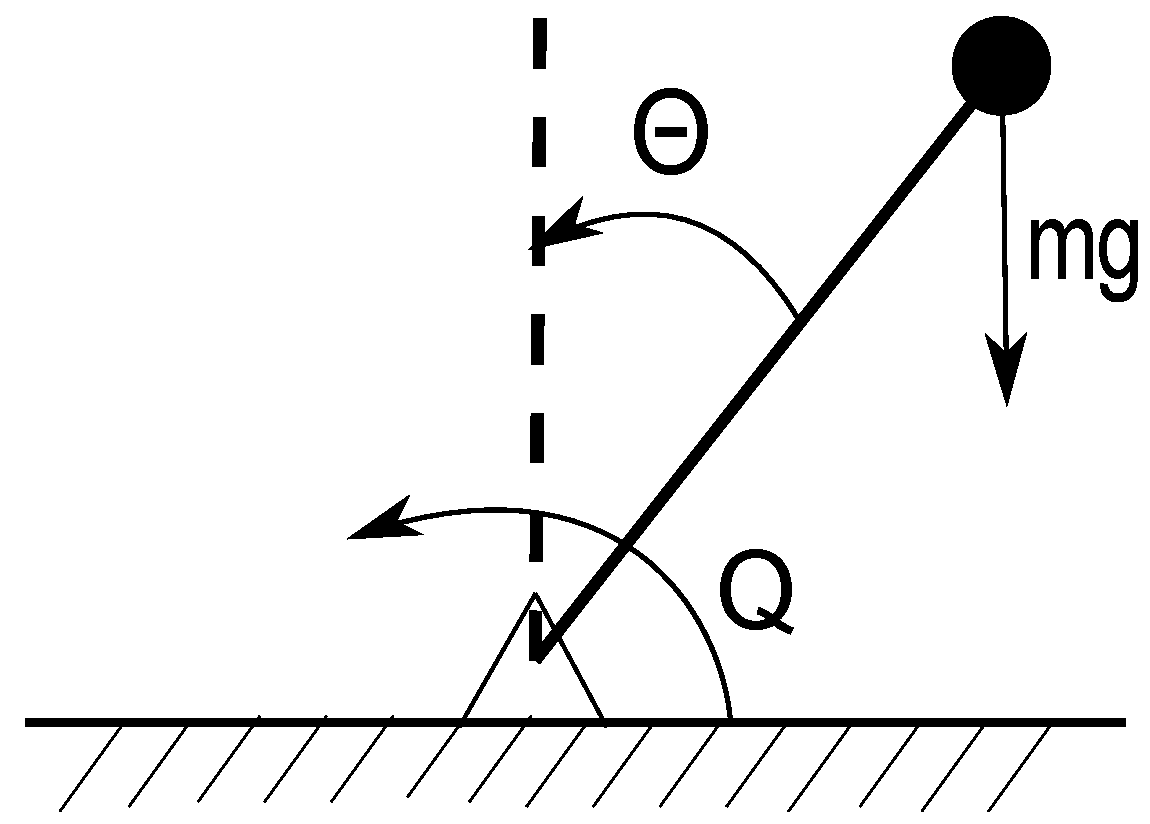
\includegraphics[width=6cm]{pendulum.pdf}
\caption{Перевернутый (обратный) маятник}
\centering
\end{figure}

Уравнение, описывающее перевернутый (обратный) маятник в окрестности $\Theta_0=0$ имеет вид
\begin{equation}\label{EQ1}
J\ddot\Theta = -Q+mgl\Theta,
\end{equation}
{\small где $\Theta$ --- угол отклонения от вертикальной оси, $Q$ --- вращательный момент, создаваемый мотором, $m$ --- масса маятника, $l$ --- длина подвеса
маятника, $J = ml^2$ --- момент инерции маятника, $g$ --- ускорение свободного падения.

Заметим, что выбор линеаризации в точке $\Theta_0$ определяется из цели управления. В данном случае цель управления --- стабилизировать маятник в положении $\Theta_0 = 0$ (задающее воздействие $g = 0$).
}

В нормальной форме уравнение \eref{EQ1} имеет вид
\begin{equation}\label{EQ1NORM}
\begin{cases}
\dot x = Ax + bu,\\
y = c x,
\end{cases}
\end{equation}
где $x = (x_1\quad x_2)^T = ( \Theta\quad \dot\Theta)^T$ --- вектор состояния системы, $A =\begin{pmatrix}0 & 1\\ \omega^2& 0\end{pmatrix}$,$b = (0\quad 1)^T$, $c = (1\quad0)$,$\omega = \sqrt{\frac{g}{l}}$, $u = -\frac{Q}{J}$ --- управление (вход) и $y = cx = x_1 = \Theta$ --- регулируемый (или измеряемый) параметр.



Используем принцип обратной связи и ПД-закон для решения задачи. Тогда
$$
u = -k_\text{п} y - k_\text{д} \dot y,
$$
где $k_\text{п}$ и $k_\text{д}$ --- коэффициенты, подлежащие определению.

Учитывая первое уравнение $\dot x_1 = x_2$ в системе \eref{EQ1NORM}, получим
$$
u = - k_\text{п} x_1 - k_\text{д} \dot x_1 = - (k_\text{п}\quad k_\text{д}) \begin{pmatrix}x_1 \\ x_2\end{pmatrix}.
$$

Подставляя это управление в \eref{EQ1NORM}, получим систему
\begin{equation}\label{EQ2}
\begin{cases}
\dot x = A_kx,\\
y = c x,
\end{cases}
\end{equation}
где $A_k = A - b(k_\text{п}\quad k_\text{д})=\begin{pmatrix}0 & 1\\ \omega^2 - k_\text{п}& - k_\text{д}\end{pmatrix}$.

Остается выбрать коэффициенты ПД-закона, исходя из устойчивости системы \eref{EQ2}. Причем добьемся этого так, чтобы в установившемся режиме не было колебаний. Это эквивалентно тому, что у характеристического полинома системы \eref{EQ2} есть только действительные отрицательные корни.

В данном случае характеристический полином замкнутой системы имеет вид
$$
\gamma(s) = \det (sI-A_k) = s^2+ k_\text{д}s+(k_\text{п}-\omega^2).
$$
Тогда выбрав $k_\text{д}$ и $k_\text{п}$ так, что $\gamma(s)$ имеет только отрицательные корни, получим устойчивую САУ и тем самым стабилизируем маятник в положении $\Theta_0 = 0$.

\begin{figure}[h]
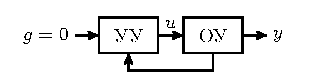
\includegraphics[width=10cm]{feedback_pendulum.pdf}
\caption{Структурная схема САУ перевернутого маятника}
\centering
\end{figure}


На схеме ОУ (маятник с мотором) описан с помощью ОДУ \eref{EQ1}, УУ (компьютер/контроллер, устанавливающий желаемый момент вращения $Q$) описывается оператором $R = k_\text{п}+k_\text{д}\frac{d}{dt}$ и реализует ПД-закон управления.

\end{document}